\documentclass[pdftex,12pt,a4paper]{article}

\usepackage{graphicx}  
\usepackage[margin=2.5cm]{geometry}
\usepackage{breakcites}
\usepackage{indentfirst}
\usepackage{pgfgantt}
\usepackage{pdflscape}
\usepackage{float}
\usepackage{epsfig}
\usepackage{epstopdf}
\usepackage[cmex10]{amsmath}
\usepackage{stfloats}
\usepackage{multirow}
\usepackage{listings}
\usepackage{tikz}
\usetikzlibrary{arrows,positioning,shapes.multipart}

\definecolor{commentgreen}{rgb}{0,0.6,0}
\definecolor{eminence}{rgb}{0.42,0.12,0.62}
\definecolor{weborange}{rgb}{1,0.49,0}

\lstdefinestyle{customasm}{
	belowcaptionskip=1\baselineskip,
	frame=single, 
	frameround=tttt,
	language=[x86masm]Assembler,
	basicstyle=\footnotesize\ttfamily,
	commentstyle=\itshape\color{green!60!black},
	keywordstyle=\color{blue!80!black},
	identifierstyle=\color{red!80!black},
	tabsize=4,
    breaklines=true,
    breakatwhitespace=false,   
    breakindent=0pt,  
	numbers=left,
	numbersep=8pt,
	stepnumber=1,
	numberstyle=\tiny\color{gray}, 
	columns = fullflexible,
}

\lstdefinestyle{customC} {
	language=C++,
	frame=single,
	frameround=tttt,
	tabsize=4,
	showstringspaces=false,
	numbers=left,
    numberstyle=\tiny\color{gray},
    breaklines=true,
    breakatwhitespace=false,   
    breakindent=0pt,   
	commentstyle=\color{commentgreen},
	keywordstyle=\color{eminence},
	stringstyle=\color{red},
	basicstyle=\footnotesize\ttfamily, % basic font setting
	emph={int,char,double,float,unsigned,void,bool},
	emphstyle={\color{blue}},
	escapechar=\&,
	classoffset=1, % starting new class
	otherkeywords={>,<,.,;,-,!,=,~},
	morekeywords={>,<,.,;,-,!,=,~},
	keywordstyle=\color{weborange},
	classoffset=0,
}

\renewcommand{\refname}{REFERENCES}
\linespread{1.3}

\usepackage{mathtools}
%\newcommand{\HRule}{\rule{\linewidth}{0.5mm}}
\thispagestyle{empty}
\begin{document}
\begin{titlepage}
\begin{center}
\textbf{}\\
\textbf{\Large{ISTANBUL TECHNICAL UNIVERSITY}}\\
\vspace{0.5cm}
\textbf{\Large{COMPUTER ENGINEERING DEPARTMENT}}\\
\vspace{2cm}
\textbf{\Large{BLG 450E\\ REAL-TIME SYSTEMS\\ ASSIGNMENT 1}}\\
\vspace{0.5cm}
\vspace{2cm}
\textbf{\Large{"Simulation Periodic and Aperiodic Scheduling Algorithms"}}\ 
\vspace{2.8cm}
\begin{table}[ht]
\centering
\Large{ 
\begin{tabular}{lcl}
\end{tabular}}
\end{table}
\vspace{1cm}

\begin{table}[ht]
\centering
\Large{ 
\begin{tabular}{rcl}
150220088  & : & ALİ EMRE ÖZCAN \ 
\end{tabular}}
\end{table}
\vspace{2.8cm}
\textbf{\Large{FALL 2025}}

\end{center}

\end{titlepage}

\thispagestyle{empty}
\addcontentsline{toc}{section}{FRONT COVER}
\addcontentsline{toc}{section}{CONTENTS}
\setcounter{tocdepth}{4}
\tableofcontents
\clearpage

\setcounter{page}{1}

\section{INTRODUCTION}

This report details the design and implementation of a C++ based simulator for various real-time scheduling algorithms. The simulator is capable of parsing task sets from input files, executing different scheduling policies, and reporting the outcome. The primary goal is to model, execute, and compare the behavior of several key scheduling algorithms in real-time systems, including Rate Monotonic (RM), Earliest Deadline First (EDF), and Least Laxity First (LLF) for periodic tasks. Additionally, the simulator supports aperiodic tasks through server mechanisms, specifically the Polling Server and the Deferrable Server. The architecture is designed to be modular, allowing for easy extension and comparison of different scheduling strategies.

\section{MATERIALS AND METHODS}
This section describes the overall architecture of the simulator, detailing the functionality of each source file and the core classes that comprise the system.

\subsection{System Architecture}
The simulator is composed of four main source files:
\begin{itemize}
    \item \textbf{rts\_parser.c/h}: A C module responsible for parsing task descriptions and server configurations from text files. It provides structs for \texttt{ParserState}, \texttt{ParsedTask}, and \texttt{ParsedServerConfig}, with support for periodic (P), dynamic (D), and aperiodic (A) task types.
    \item \textbf{task\_ali.cpp}: Defines the fundamental data structures, \texttt{Task} and \texttt{Job}, which represent the tasks to be scheduled and their individual instances. Uses C++ smart pointers (\texttt{shared\_ptr}) for efficient memory management.
    \item \textbf{schedule\_ali.cpp}: Contains the implementation of the scheduling algorithms themselves. It features a class hierarchy with an abstract \texttt{Scheduler} base class and concrete implementations for RM, DM, EDF, LLF, Polling Server, and Deferrable Server.
    \item \textbf{run\_ali.cpp}: The main driver of the simulation. It orchestrates the process of parsing, scheduling, and printing the results. Provides two simulation modes: \texttt{runPeriodicSimulation} for periodic-only tasks and \texttt{runAperiodicSimulation} for mixed workloads with server mechanisms.
\end{itemize}

The compilation process uses a \texttt{Makefile} to coordinate building the C parser module and linking it with the C++ scheduling components. The parser is compiled separately as an object file (\texttt{rts\_parser.o}) and linked with the main C++ executable.

\subsection{Class Relationship Diagram}
The relationship between the main classes is shown in Figure~\ref{fig:class_diagram}. The \texttt{Scheduler} class acts as an abstract base for all concrete scheduling algorithms, which inherit from it. A \texttt{Job} is linked to a parent \texttt{Task} (a "has-a" relationship) and the schedulers operate on a collection of jobs.

\begin{figure}[H]
    \centering
    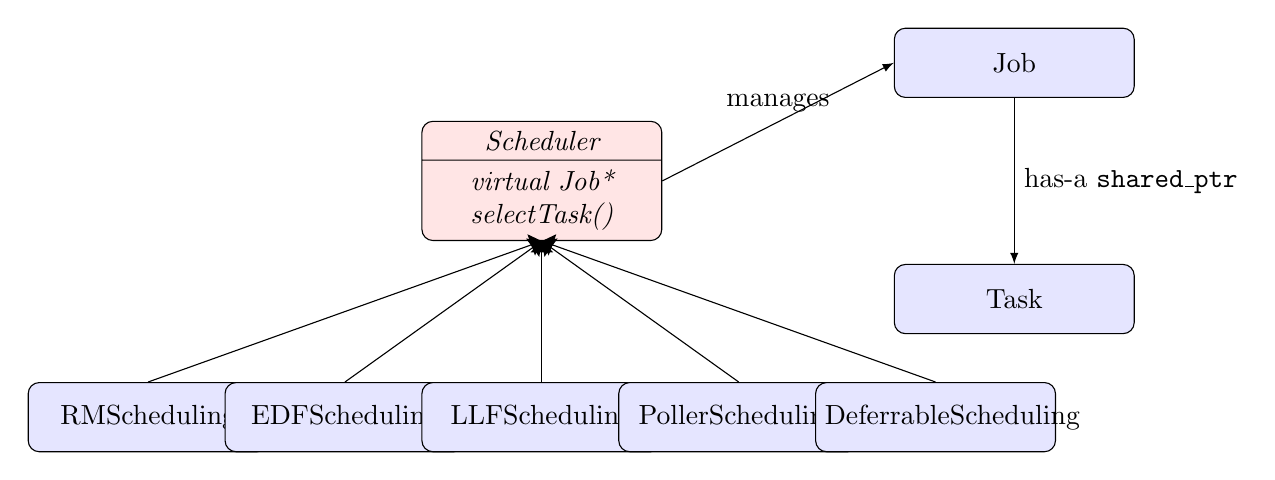
\begin{tikzpicture}[
        auto,
        class/.style={
            rectangle, 
            draw=black, 
            fill=blue!10, 
            text width=8em, 
            text centered, 
            minimum height=2.5em,
            rounded corners
        },
        abstract/.style={
            class,
            font=\itshape,
            fill=red!10,
            rectangle split,
            rectangle split parts=2
        },
        arrow/.style={-latex, draw},
        inheritance/.style={-triangle 90, draw}
    ]
        % Class Nodes
        \node[abstract] (scheduler) at (0,0) {Scheduler \nodepart{two} virtual Job* selectTask()};
        
        \node[class] (rm) at (-5,-3) {RMScheduling};
        \node[class] (edf) at (-2.5,-3) {EDFScheduling};
        \node[class] (llf) at (0,-3) {LLFScheduling};
        \node[class] (poller) at (2.5,-3) {PollerScheduling};
        \node[class] (defer) at (5,-3) {DeferrableScheduling};
        
        \node[class] (job) at (6,1.5) {Job};
        \node[class] (task) at (6,-1.5) {Task};

        % Inheritance lines
        \draw[inheritance] (rm.north) -- (scheduler.south);
        \draw[inheritance] (edf.north) -- (scheduler.south);
        \draw[inheritance] (llf.north) -- (scheduler.south);
        \draw[inheritance] (poller.north) -- (scheduler.south);
        \draw[inheritance] (defer.north) -- (scheduler.south);
        
        % Association lines
        \draw[arrow] (job.south) -- (task.north) node[midway, right] {has-a \texttt{shared\_ptr}};
        \draw[arrow] (scheduler.east) -- (job.west) node[midway, above] {manages};

    \end{tikzpicture}
    \caption{Class diagram showing the main relationships.}
    \label{fig:class_diagram}
\end{figure}

\subsection{File Parsing: \texttt{rts\_parser.c}}
This module provides the functionality to read and interpret text files that define the task set for the simulation. It is written in C for straightforward file I/O and string manipulation, then interfaced with C++ code through the \texttt{extern "C"} mechanism.

The primary function, \texttt{parse\_file}, reads a file line by line. Each line is parsed to identify the task type (Periodic 'P', Aperiodic 'A', or Dynamic 'D') or server configuration rules. The parsed data is stored in a \texttt{ParserState} struct, which holds an array of \texttt{ParsedTask} structs and a \texttt{ParsedServerConfig} struct.

\subsubsection{Parser Data Structures}
The parser header (\texttt{rts\_parser.h}) defines several key structures:

\begin{lstlisting}[style=customC, caption={Parser data structures}, label=parser_structs]
// Maximum limits
#define MAX_TASKS 50
#define MAX_LINE_LENGTH 256

// Task types
typedef enum {
    PARSED_TASK_PERIODIC,
    PARSED_TASK_DYNAMIC,
    PARSED_TASK_APERIODIC
} ParsedTaskType;

// Individual task representation
typedef struct {
    ParsedTaskType type;
    int release_time;
    int execution_time;
    int period;
    int deadline;
} ParsedTask;

// Server types
typedef enum {
    SERVER_NONE,
    SERVER_POLLER,
    SERVER_DEFERRABLE
} ParsedServerType;

// Server configuration
typedef struct {
    ParsedServerType type;
    int budget;
    int period;
    ParsedSchedulingType scheduling; // RM or EDF
} ParsedServerConfig;

// Complete parser state
typedef struct {
    ParsedTask tasks[MAX_TASKS];
    int task_count;
    ParsedServerConfig server;
} ParserState;
\end{lstlisting}

\subsubsection{Input File Format}
The parser makes the following assumptions about the input file format:
\begin{itemize}
    \item Each line contains a single task definition or a configuration rule.
    \item Lines starting with a '\#' character are treated as comments and are ignored.
    \item Empty or whitespace-only lines are ignored.
    \item Parameters on a line are separated by spaces or tabs.
    \item \textbf{Periodic Task (P):} Defined with the format \texttt{P [ri] ei pi [di]} where:
    \begin{itemize}
        \item \texttt{ri}: Release time (optional, defaults to 0)
        \item \texttt{ei}: Execution time (required)
        \item \texttt{pi}: Period (required)
        \item \texttt{di}: Relative deadline (optional, defaults to period)
    \end{itemize}
    The parser accepts three formats: \texttt{P ei pi}, \texttt{P ri ei pi}, or \texttt{P ri ei pi di}.

    \item \textbf{Dynamic Task (D):} Defined with the format \texttt{D ei pi di} (execution time, period, deadline). Dynamic tasks always start at time 0.

    \item \textbf{Aperiodic Task (A):} Defined with the format \texttt{A ri ei} (release time, execution time). Aperiodic tasks have no period and no hard deadline.

    \item \textbf{Server Configuration (S):} Defined with the format \texttt{S es ps TYPE SCHEDULING} where:
    \begin{itemize}
        \item \texttt{es}: Server budget (execution capacity per period)
        \item \texttt{ps}: Server replenishment period
        \item \texttt{TYPE}: Either \texttt{POLLER} or \texttt{DEFERABLE}
        \item \texttt{SCHEDULING}: Either \texttt{RM} (Rate Monotonic) or \texttt{EDF} (Earliest Deadline First)
    \end{itemize}
\end{itemize}

\subsubsection{Input Configuration Examples}
Below are concrete examples of input files that the simulator can process.

\paragraph{Example 1: Periodic Tasks Only}
\begin{lstlisting}[style=customC, caption={example\_periodic.txt: Testing RM/EDF/LLF}, label=ex_periodic]
# Example periodic tasks for RM/EDF/LLF testing
# Format: P ei pi (execution_time, period)
# Implicit: release_time=0, deadline=period

D 2 6 4
D 1 4 6
P 3 12
\end{lstlisting}

This configuration defines two dynamic tasks with explicit deadlines different from their periods (D tasks allow deadline $\neq$ period), and one standard periodic task. The simulator will run RM, DM, EDF, and LLF algorithms on this task set.

\paragraph{Example 2: Mixed Periodic and Aperiodic Tasks}
\begin{lstlisting}[style=customC, caption={example\_aperiodic.txt: Testing server mechanisms}, label=ex_aperiodic]
# Example with periodic and aperiodic tasks
# Testing Poller/Deferrable servers

# Periodic tasks
P 6 24
P 1 8
P 2 12

# Aperiodic tasks
A 1 5
A 3 8

# Server configuration: budget=2, period=6, Deferrable, RM scheduling
S 2 6 DEFERABLE RM
\end{lstlisting}

This configuration includes three periodic tasks, two aperiodic tasks arriving at times 1 and 3, and a Deferrable Server with a budget of 2 time units replenished every 6 time units, using Rate Monotonic scheduling for periodic tasks.

\begin{lstlisting}[style=customC, caption={Parsing a periodic task in \texttt{rts\_parser.c}}, label=parse_periodic]
// Parse periodic task: P ri ei pi di OR P ri ei pi OR P ei pi
static int parse_periodic_task(char *line, ParserState *state) {
    ParsedTask task;
    task.type = PARSED_TASK_PERIODIC;

    int values[4];
    int count = 0;
    char *token = strtok(line, " \t");

    // Skip 'P'
    token = strtok(NULL, " \t");

    // Read all numeric values
    while (token != NULL && count < 4) {
        values[count++] = atoi(token);
        token = strtok(NULL, " \t");
    }

    if (count == 2) {
        // Format: P ei pi
        task.release_time = 0;
        task.execution_time = values[0];
        task.period = values[1];
        task.deadline = values[1];  // Implicit deadline = period
    } else if (count == 4) {
        // Format: P ri ei pi di
        task.release_time = values[0];
        task.execution_time = values[1];
        task.period = values[2];
        task.deadline = values[3];
    } else {
        fprintf(stderr, "Error: Invalid periodic task format...\n");
        return -1;
    }

    state->tasks[state->task_count++] = task;
    return 0;
}
\end{lstlisting}

\subsection{Core Data Structures: \texttt{task\_ali.cpp}}
This file establishes the object-oriented foundation for the simulation. It makes a key distinction between a task and a job, which is fundamental to real-time systems.

\subsubsection{Task Types and Enumerations}
The implementation defines several enumeration types to categorize tasks and servers:

\begin{lstlisting}[style=customC, caption={Task and Server type enumerations}, label=enum_types]
enum TaskTypes {Periodic, Dynamic, Aperiodic};
enum ServerTypes {None, Background, Poller, Defferable};
\end{lstlisting}

These enumerations provide type safety and clarity when working with different task categories throughout the codebase.

\subsubsection{The Task Class}
In real-time systems, a \textbf{Task} is a blueprint for a recurring piece of work. It defines the rules, such as timing constraints, but is not the work itself. The \texttt{Task} class represents this blueprint. Its properties are constant for all work generated by it:
\begin{itemize}
    \item \texttt{id}: A unique identifier, automatically assigned using a static counter (\texttt{num\_tasks}).
    \item \texttt{type}: The task category (Periodic, Dynamic, or Aperiodic).
    \item \texttt{exec\_time}: The worst-case execution time (WCET) required to complete one instance of the task.
    \item \texttt{per} (Period): The rate at which the task generates work. For periodic tasks, this is the interval between job releases.
    \item \texttt{rel\_time}: The initial release time offset for the task.
    \item \texttt{deadline}: The relative deadline by which an instance of the task must complete its execution.
    \item \texttt{server}: The type of server associated with the task (if any).
\end{itemize}
This class acts as a static configuration for a type of work in the system.

\begin{lstlisting}[style=customC, caption={The Task class definition.}, label=task_class]
class Task {
private:
    static int num_tasks;  // Static counter for unique IDs
    int id;
    TaskTypes type;
    double exec_time;
    double per;
    double rel_time;
    double deadline;
    ServerTypes server;
public:
    Task(TaskTypes t, double e, double p = 0, double r = 0,
         double d = 0, ServerTypes s = None)
        : id(++num_tasks), type(t), exec_time(e), per(p),
          rel_time(r), server(s) {
            if(d > 0) deadline = d;
            else deadline = p; // Implicit deadline = period
        }

    // Accessor methods
    int getId() {return id;}
    TaskTypes getType() {return type;}
    double getE() {return exec_time;}
    double getP() {return per;}
    double getD() {return deadline;}
    double getR() {return rel_time;}
    ServerTypes getServer() {return server;}
};

// Static member initialization
int Task::num_tasks = 0;
\end{lstlisting}

The use of a static counter ensures each task receives a unique ID, which is critical for tracking and debugging during simulation.

\subsubsection{The Job Class}
A \textbf{Job} is a specific instance of a task that is ready to be executed by the CPU. For a periodic task, a new job is created at the start of each period. The \texttt{Job} class tracks the dynamic state of one specific instance of work.

Key properties include:
\begin{itemize}
    \item \texttt{shared\_ptr\textless{}Task\textgreater{} task}: This C++ smart pointer links a \texttt{Job} to its parent \texttt{Task}. Using a \texttt{shared\_ptr} is memory-efficient because many jobs can point to the same single \texttt{Task} object without copying its data. It also automatically manages memory through reference counting, preventing leaks by deleting the \texttt{Task} object only when no \texttt{Job} objects are pointing to it anymore. This is a crucial application of RAII (Resource Acquisition Is Initialization) in modern C++.
    \item \texttt{rem}: The remaining execution time. This is critical for preemption. When a job is paused, the scheduler must know how much time it still needs to finish when it gets the CPU again. Initially set to the task's execution time.
    \item \texttt{started}: A boolean flag indicating whether the job has begun execution. Useful for tracking job state transitions.
    \item \texttt{abs\_deadline}: The absolute deadline in the simulation timeline, calculated as \texttt{job\_release\_time + task->getD()}. Dynamic schedulers like EDF use this exact time to decide which job to run next.
    \item \texttt{job\_release\_time}: The exact time at which this job was released into the ready queue.
\end{itemize}

\begin{lstlisting}[style=customC, caption={The Job class definition.}, label=job_class]
class Job {
private:
    std::shared_ptr<Task> task;  // Smart pointer to parent Task
    double rem;                   // Remaining execution time
    bool started;                 // Has job started execution?
    double abs_deadline;          // Absolute deadline
    double job_release_time;      // Release time of this job
public:
    Job(std::shared_ptr<Task> t, double release_time)
        : task(t), rem(t->getE()), abs_deadline(release_time + t->getD()),
          job_release_time(release_time), started(false) {
    }

    // Accessor methods
    std::shared_ptr<Task> getTask() {return task;}
    double getRem() {return rem;}
    double getAbsDeadline() {return abs_deadline;}
    double getJobReleaseTime() {return job_release_time;}
    bool hasStarted() {return started;}

    // Check if job is complete
    bool isComplete() {return rem <= 0;}

    // Execute the job for a given time
    double execute(double time) {
        if(rem > 0) {
            started = true;
            if (rem - time < 0) {
                double tmp = rem;
                rem = 0;
                return tmp;  // Return actual time executed
            }
            else {
                rem = rem - time;
                return time;
            }
        }
        return 0;
    }
};
\end{lstlisting}

The \texttt{execute} method is particularly important: it decrements the remaining time by the specified amount, marks the job as started, and returns the actual execution time consumed. This allows for proper handling of scenarios where the remaining execution time is less than the requested execution time.

\subsection{Scheduling Algorithms: \texttt{schedule\_ali.cpp}}
This file contains the logic for the different scheduling policies, using C++ polymorphism to create a flexible and extensible design.

\subsubsection{Abstract Scheduler Class and Polymorphism}
\texttt{Scheduler} is an abstract base class. It acts as a contract, defining a common interface that all schedulers must follow. This allows the main simulation loop to treat all schedulers the same way, without needing to know which specific algorithm is being used.

\begin{lstlisting}[style=customC, caption={The abstract Scheduler class.}, label=scheduler_class]
class Scheduler {
private:
    string name;
    double curr_time;
    vector<tuple<double, Job*>> logs;  // Execution timeline
    vector<Job*> finished_jobs;
    vector<Job*> missed_deadlines;

public:
    Scheduler(string n) : name(n), curr_time(0) {}

    // Time management
    void clockTick(double t) { curr_time = curr_time + t; }
    double getCurrentTime() { return curr_time; }

    // Logging and tracking
    void addLog(Job* job) { logs.push_back({curr_time, job}); }
    void addFinishedJob(Job* job) { finished_jobs.push_back(job); }
    void addMissedDeadline(Job* job) { missed_deadlines.push_back(job); }

    // Getters for results
    vector<tuple<double, Job*>> getLogs() { return logs; }
    vector<Job*> getFinishedJobs() { return finished_jobs; }
    vector<Job*> getMissedDeadlines() { return missed_deadlines; }
    string getName() { return name; }

    // Pure virtual function - must be implemented by subclasses
    virtual Job* selectTask(vector<Job*> queue) = 0;

    // Virtual functions with default implementations for servers
    virtual double budgetReplenishment() { return 0; }
    virtual double budgetConsumption(double exec) { return 0; }
    virtual void execute_server_version(Job* job, double t) {
        if(job) job->execute(t);
    }
    virtual double getReplenishmentPeriod() { return 0; }
};
\end{lstlisting}

The \texttt{Scheduler} class provides:
\begin{itemize}
    \item \textbf{State management}: Tracks current simulation time, execution logs, completed jobs, and deadline violations.
    \item \textbf{Logging infrastructure}: The \texttt{logs} vector stores tuples of \texttt{\textless{}time, Job*\textgreater{}} to create a complete execution timeline for visualization and analysis.
    \item \textbf{Pure virtual \texttt{selectTask}}: The line \texttt{virtual Job* selectTask(...) = 0;} declares a \textbf{pure virtual function}. The \texttt{virtual} keyword enables \textbf{polymorphism} - when the simulation code calls \texttt{scheduler->selectTask()}, C++ dynamically dispatches to the correct implementation at runtime (RM, EDF, LLF, etc.). The \texttt{= 0} makes it "pure," forcing every derived class to implement its own scheduling logic.
    \item \textbf{Server support}: Virtual functions like \texttt{budgetReplenishment} and \texttt{budgetConsumption} provide default implementations (returning 0) for non-server schedulers, while server-based schedulers override them with actual budget management logic.
\end{itemize}

This design pattern exemplifies the \textbf{Template Method} and \textbf{Strategy} patterns, enabling algorithm extensibility without modifying the simulation loop.

\subsubsection{Periodic Schedulers}
These schedulers are designed for tasks that arrive at regular intervals. Each implements the \texttt{selectTask} method with its own priority calculation logic.

\paragraph{RMScheduling (Rate Monotonic):} This is a \textbf{static-priority} algorithm. In RM, priority is based on the task's period: the shorter the period, the higher the priority. Priorities are assigned once and never change. RM is the optimal static-priority algorithm: if a set of tasks cannot be scheduled by RM, no other static-priority algorithm can schedule it either.

\begin{lstlisting}[style=customC, caption={Rate Monotonic task selection}, label=rm_select]
class RMScheduling : public Scheduler {
public:
    RMScheduling() : Scheduler("Rate Monotonic") {}

    Job* selectTask(vector<Job*> queue) {
        if (queue.empty()) return NULL;

        Job* highest = queue.front();
        for(int i = 1; i < queue.size(); i++) {
            // Shorter period = higher priority
            if(queue[i]->getTask()->getP() < highest->getTask()->getP())
                highest = queue[i];
        }
        return highest;
    }
};
\end{lstlisting}

\paragraph{EDFScheduling (Earliest Deadline First):} This is a \textbf{dynamic-priority} algorithm. Priority is determined at runtime based on the job's absolute deadline. The job with the closest deadline gets the highest priority. EDF is \textbf{optimal} on a single processor: if a set of tasks can be scheduled by any algorithm, EDF can schedule it successfully.

\begin{lstlisting}[style=customC, caption={EDF task selection}, label=edf_select]
class EDFScheduling : public Scheduler {
public:
    EDFScheduling() : Scheduler("Earliest Deadline First") {}

    Job* selectTask(vector<Job*> queue) {
        if (queue.empty()) return NULL;

        Job* highest = queue.front();
        for(int i = 1; i < queue.size(); i++) {
            // Earlier absolute deadline = higher priority
            if(queue[i]->getAbsDeadline() < highest->getAbsDeadline())
                highest = queue[i];
        }
        return highest;
    }
};
\end{lstlisting}

\paragraph{LLFScheduling (Least Laxity First):} This is another optimal, dynamic-priority algorithm. Laxity is the "slack time" a job has before it will miss its deadline (\texttt{deadline - current\_time - remaining\_execution}). The job with the least slack gets the highest priority. While optimal, LLF is less common in practice than EDF because it has higher overhead; priorities can change more frequently.

\begin{lstlisting}[style=customC, caption={LLF task selection}, label=llf_select]
class LLFScheduling : public Scheduler {
public:
    LLFScheduling() : Scheduler("Least Laxity First") {}

    Job* selectTask(vector<Job*> queue) {
        if (queue.empty()) return NULL;

        Job* highest = queue.front();
        double curr = getCurrentTime();
        for(int i = 1; i < queue.size(); i++) {
            double laxity_i = queue[i]->getAbsDeadline() - curr
                            - queue[i]->getRem();
            double laxity_highest = highest->getAbsDeadline() - curr
                                  - highest->getRem();
            if(laxity_i < laxity_highest)
                highest = queue[i];
        }
        return highest;
    }
};
\end{lstlisting}

The implementation also includes \textbf{DMScheduling (Deadline Monotonic)}, which is similar to RM but uses relative deadlines instead of periods for static priority assignment. DM is optimal when deadlines are less than or equal to periods.

\subsubsection{Aperiodic Server Schedulers in Detail}
Aperiodic tasks arrive unpredictably. To handle them without causing periodic tasks to miss their deadlines, we use a \textbf{server}. A server is a special, high-priority periodic task that runs aperiodic jobs instead of its own work. It is given a limited \texttt{budget} of execution time every \texttt{replenishment\_period}. This section explains the implementation of the two servers in detail.

\paragraph{Polling Server}
This is a simple server. It gets its full budget at the start of each period. If aperiodic jobs are waiting, it serves them using its budget. If a higher-priority periodic job preempts it, or if there are no aperiodic jobs to run, \textbf{any unused budget is lost}. This can lead to poor response times if an aperiodic job arrives just after the budget has been discarded.

\subparagraph{Budget Replenishment:}
The budget is refilled to its maximum capacity at the start of each replenishment period. This is checked at every time step using the modulo operator. The small epsilon (\texttt{0.01}) handles floating-point inaccuracies.
\begin{lstlisting}[style=customC, caption={Polling Server Budget Replenishment}]
double budgetReplenishment() {
    // Check if the current time is the start of a new replenishment period
    if(std::fmod(getCurrentTime(), rep_period) < 0.01) {
        // Refill the budget
        rem_budget = budget;
    }
    return rem_budget;
}
\end{lstlisting}

\subparagraph{Task Selection:}
The server's priority is handled like a periodic task with a period equal to \texttt{rep\_period}. When selecting a task, it first checks if it has any budget.
\begin{itemize}
    \item \textbf{If budget > 0 and aperiodic jobs exist:} It tentatively selects the first aperiodic job (First-Come, First-Served). However, it must respect the priority of periodic tasks. It checks if the highest-priority periodic job (shortest period) has a higher priority than the server itself (\texttt{highest\_periodic->getP() < rep\_period}). If so, the periodic job is chosen, and the polling server's budget is immediately discarded (\texttt{rem\_budget = 0}).
    \item \textbf{If no budget, or no aperiodic jobs:} It ignores aperiodic tasks and simply selects the highest-priority periodic job according to Rate Monotonic (RM) logic. If the server was idle, it also discards any remaining budget.
\end{itemize}

\begin{lstlisting}[style=customC, caption={Polling Server Task Selection Logic}]
Job* PollerScheduling::selectTask(vector<Job*> q) {
    // ... split queue into periodic and aperiodic ...

    if (rem_budget > 0) {
        if (!aper_queue.empty()) {
            highest = aper_queue.front(); // Tentatively select aperiodic job

            if (!queue.empty()) {
                Job* highest_periodic = ... // Find highest-priority periodic (RM)
                
                // If periodic task has higher priority than the server
                if (highest_periodic->getTask()->getP() < rep_period) {
                    highest = highest_periodic; // Periodic job preempts
                    rem_budget = 0;  // IMPORTANT: Polling server discards budget
                }
            }
        } else if (!queue.empty()) {
            rem_budget = 0;  // No aperiodic jobs, discard budget and run periodic
            highest = ... // Find highest-priority periodic (RM)
        }
    } else { // No budget
        // Run highest-priority periodic task
        highest = ... 
    }
    return highest;
}
\end{lstlisting}

\paragraph{Deferrable Server}
This server improves on the Polling Server. It also gets a budget periodically, but if it is preempted by a periodic task, it \textbf{preserves its budget}. This allows it to service aperiodic requests more quickly as soon as the CPU becomes available again, leading to better average response time.

\subparagraph{Budget Replenishment:}
The replenishment logic is identical to the Polling Server's. The budget is refilled at the start of each period.
\begin{lstlisting}[style=customC, caption={Deferrable Server Budget Replenishment}]
double budgetReplenishment() {
    if(std::fmod(getCurrentTime(), rep_period) < 0.01) {
        rem_budget = budget;
    }
    return rem_budget;
}
\end{lstlisting}

\subparagraph{Task Selection:}
The logic is similar to the Polling Server, but with one critical difference.
\begin{itemize}
    \item \textbf{If budget > 0 and aperiodic jobs exist:} It tentatively selects the aperiodic job. If a higher-priority periodic job exists, that job runs, but the Deferrable Server \textbf{does not discard its budget}. The budget is "deferred" to be used later.
    \item \textbf{If no budget, or no aperiodic jobs:} It runs the highest-priority periodic job. The budget is also preserved.
\end{itemize}
This preservation of budget is the key advantage of the Deferrable Server.

\begin{lstlisting}[style=customC, caption={Deferrable Server Task Selection Logic}]
Job* DeferrableScheduling::selectTask(vector<Job*> q) {
    // ... split queue ...

    if (rem_budget > 0) {
        if (!aper_queue.empty()) {
            highest = aper_queue.front(); // Tentatively select aperiodic job

            if (!queue.empty()) {
                Job* highest_periodic = ... // Find highest-priority periodic (RM)
                
                // If periodic task has higher priority than the server
                if (highest_periodic->getTask()->getP() < rep_period) {
                    highest = highest_periodic; // Periodic job preempts
                    // *** KEY DIFFERENCE: Budget is NOT discarded ***
                }
            }
        } else if (!queue.empty()) {
            // Run periodic, but keep the budget for later
            highest = ... // Find highest-priority periodic (RM)
        }
    } else { // No budget
        highest = ... // Run highest-priority periodic
    }
    return highest;
}
\end{lstlisting}

\subparagraph{Budget Consumption:}
Another key difference lies in how the budget is consumed. The Deferrable Server only consumes the amount of budget it actually uses. The Polling Server, in this implementation, consumes its entire remaining budget in one go.
\begin{lstlisting}[style=customC, caption={Deferrable Server Budget Consumption}]
double DeferableScheduling::budgetConsumption(double exec) {
    double consumed = 0;
    if(rem_budget > 0) {
        if(rem_budget > exec) { // If there is enough budget
            consumed = exec;
            rem_budget = rem_budget - exec; // Only subtract what was used
        } else { // If not enough budget
            consumed = rem_budget; // Use up all the remaining budget
            rem_budget = 0;
        }
    }
    return consumed;
}
\end{lstlisting}

\subsection{Simulation Driver: \texttt{run\_ali.cpp}}
This file serves as the entry point and orchestrates the entire simulation. Its \texttt{main} function manages the high-level control flow and coordinates between the C parser and C++ scheduler components.

\subsubsection{C and C++ Integration}
The simulation driver bridges C and C++ code using the \texttt{extern "C"} linkage mechanism:

\begin{lstlisting}[style=customC, caption={C/C++ integration}, label=c_cpp_link]
extern "C" {
#include "rts_parser.h"
}

// Helper function to convert parsed tasks into C++ Task objects
void loadTasksFromParser(ParserState* state,
                         vector<shared_ptr<Task>>& tasks) {
    tasks.clear();
    for (int i = 0; i < state->task_count; i++) {
        ParsedTask* p_task = &state->tasks[i];
        TaskTypes type;

        if (p_task->type == PARSED_TASK_PERIODIC) {
            type = Periodic;
        } else if (p_task->type == PARSED_TASK_DYNAMIC) {
            type = Dynamic;
        } else {
            type = Aperiodic;
        }

        tasks.push_back(make_shared<Task>(
            type,
            (double)p_task->execution_time,
            (double)p_task->period,
            (double)p_task->release_time,
            (double)p_task->deadline
        ));
    }
}
\end{lstlisting}

This function converts C structs from the parser into C++ \texttt{shared\_ptr\textless{}Task\textgreater{}} objects, performing type conversions and mapping between the C enum types and C++ enum types.

\subsubsection{Main Control Flow}
The key steps are:
\begin{enumerate}
    \item \textbf{Parse Arguments}: The program checks for command-line arguments, which are treated as paths to input files. The usage is: \texttt{./run\_ali.exe \textless{}file1\textgreater{} [file2] ...}
    \item \textbf{Process Files}: For each file, it:
    \begin{itemize}
        \item Initializes the C parser state (\texttt{init\_parser\_state})
        \item Parses the file (\texttt{parse\_file})
        \item Prints parsed tasks and server configuration
        \item Converts C-style parsed data into C++ objects using \texttt{loadTasksFromParser}
    \end{itemize}
    \item \textbf{Run Simulations}: Based on whether a server is defined, it invokes:
    \begin{itemize}
        \item \texttt{runPeriodicSimulation}: For task sets with only periodic tasks. Runs RM, DM, EDF, and LLF simulations sequentially, each with a simulation length of 50 time units.
        \item \texttt{runAperiodicSimulation}: For mixed task sets. Runs the specified server (Polling or Deferrable) with the configured scheduling algorithm (RM or EDF).
    \end{itemize}
    \item \textbf{Print Results}: The \texttt{printSchedule} function formats and prints the execution log, including a summary of completed jobs and missed deadlines.
\end{enumerate}

\subsubsection{Simulation Loop Implementation}
The simulation loop advances time in discrete steps (typically 1.0 time unit), performing the following actions at each step:
\begin{enumerate}
    \item \textbf{Job Release}: Check if any periodic tasks need to release new jobs (when current time is a multiple of the period).
    \item \textbf{Deadline Check}: Scan the ready queue for jobs whose absolute deadline has passed and log them as missed deadlines.
    \item \textbf{Task Selection}: Call the scheduler's polymorphic \texttt{selectTask} method.
    \item \textbf{Execution}: Execute the selected job for one time unit, updating its remaining time.
    \item \textbf{Completion}: Remove finished jobs from the queue and log them.
    \item \textbf{Time Advance}: Increment the simulation clock.
\end{enumerate}

\begin{lstlisting}[style=customC, caption={Periodic simulation loop from \texttt{runPeriodicSimulation}}, label=sim_loop]
void runPeriodicSimulation(const string& name,
                           const vector<shared_ptr<Task>>& tasks,
                           double sim_length) {
    Scheduler* sch = nullptr;
    if (name == "RM") sch = new RMScheduling();
    else if (name == "EDF") sch = new EDFScheduling();
    else if (name == "LLF") sch = new LLFScheduling();
    else if (name == "DM") sch = new DMScheduling();

    vector<Job> all_jobs;
    all_jobs.reserve(1000);  // Pre-allocate for efficiency
    vector<Job*> queued_jobs;

    while (sch->getCurrentTime() < sim_length) {
        double current_time = sch->getCurrentTime();

        // 1. Release new jobs for periodic/dynamic tasks
        for (const auto& task : tasks) {
            if (task->getType() == Periodic || task->getType() == Dynamic) {
                // Use fmod to check period alignment with epsilon tolerance
                if (fmod(current_time, task->getP()) < 0.01
                    && current_time >= task->getR()) {
                    all_jobs.emplace_back(task, current_time);
                    queued_jobs.push_back(&all_jobs.back());
                }
            }
        }

        // 2. Check for deadline misses
        for (auto it = queued_jobs.begin(); it != queued_jobs.end();) {
            if ((*it)->getAbsDeadline() <= current_time) {
                sch->addMissedDeadline(*it);
                it = queued_jobs.erase(it);
            } else {
                it++;
            }
        }

        // 3. Select and execute job
        Job* now = sch->selectTask(queued_jobs);
        if (now) {
            now->execute(1.0);
            sch->addLog(now);

            if (now->isComplete()) {
                queued_jobs.erase(remove(queued_jobs.begin(),
                                        queued_jobs.end(), now),
                                queued_jobs.end());
                sch->addFinishedJob(now);
            }
        } else {
            sch->addLog(nullptr);  // Log IDLE time
        }

        // 4. Advance simulation clock
        sch->clockTick(1.0);
    }

    printSchedule(sch);
    delete sch;
}
\end{lstlisting}

Key implementation details:
\begin{itemize}
    \item \textbf{Floating-point tolerance}: Uses \texttt{fmod(current\_time, task->getP()) < 0.01} to handle floating-point precision issues when checking if it's time to release a new job.
    \item \textbf{Memory management}: Uses \texttt{vector\textless{}Job\textgreater{}} to store all jobs and \texttt{vector\textless{}Job*\textgreater{}} for the ready queue. The \texttt{reserve(1000)} call pre-allocates memory to avoid repeated reallocations.
    \item \textbf{Polymorphic dispatch}: \texttt{sch->selectTask(queued\_jobs)} calls the appropriate scheduler implementation through virtual function dispatch.
    \item \textbf{Idle time logging}: When \texttt{selectTask} returns \texttt{nullptr}, the simulator logs \texttt{nullptr} to indicate the CPU was idle at that time step.
\end{itemize}

The \texttt{runAperiodicSimulation} function is similar but includes additional logic for:
\begin{itemize}
    \item One-time release of aperiodic tasks at their specified arrival times
    \item Server budget replenishment (\texttt{sch->budgetReplenishment()})
    \item Server-aware execution (\texttt{sch->execute\_server\_version()})
\end{itemize}

\section{RESULTS AND DISCUSSION}
The program successfully simulates the specified scheduling algorithms. When executed with an input file, it produces a textual schedule trace for each relevant algorithm. The output shows the timeline of execution, indicating which task (if any) is running at each time step. It also provides a summary of performance, including the total number of completed jobs and, crucially, the number of missed deadlines.

\subsection{Output Format and Structure}
The simulator produces structured output with the following components:
\begin{enumerate}
    \item \textbf{Parsed Task Information}: Shows all tasks read from the input file with their parameters.
    \item \textbf{Server Configuration}: If applicable, displays server type, budget, period, and scheduling algorithm.
    \item \textbf{Execution Timeline}: A chronological log showing which task executes at each time step.
    \item \textbf{Summary Statistics}: Final counts of completed jobs and missed deadlines.
\end{enumerate}

\subsection{Example Output: Periodic Tasks}
Below is a sample output for the \texttt{example\_periodic.txt} file running under Rate Monotonic scheduling:

\begin{lstlisting}[style=customC, caption={Sample output for RM scheduling}, label=output_rm]
========== Processing file: example_periodic.txt ==========

=== Parsed Tasks ===
Total tasks: 3

Task 1 (Dynamic):
  Release: 0, Exec: 2, Period: 6, Deadline: 4.000000

Task 2 (Dynamic):
  Release: 0, Exec: 1, Period: 4, Deadline: 6.000000

Task 3 (Periodic):
  Release: 0, Exec: 3, Period: 12, Deadline: 12.000000


--- Running Periodic Simulation: RM ---

=== Rate Monotonic Scheduling ===
Time    Task    Action
----    ----    ------
0       T2(D)   Executing (deadline: 6.00)
1       T1(D)   Executing (deadline: 4.00)
3       T3(P)   Executing (deadline: 12.00)
4       T2(D)   Executing (deadline: 10.00)
5       T3(P)   Executing (deadline: 12.00)
6       T1(D)   Executing (deadline: 10.00)
8       T2(D)   Executing (deadline: 14.00)
9       T3(P)   Executing (deadline: 12.00)
10      IDLE    -
12      T2(D)   Executing (deadline: 18.00)
13      T1(D)   Executing (deadline: 16.00)
15      T3(P)   Executing (deadline: 24.00)

Summary:
Completed jobs: 15
Missed deadlines: 0
\end{lstlisting}

This output demonstrates several key behaviors:
\begin{itemize}
    \item \textbf{Priority ordering}: Task T2 (period=4) has the highest priority, followed by T1 (period=6), then T3 (period=12). This is evident at time 0, where T2 executes first despite multiple tasks being ready.
    \item \textbf{Preemption}: At time 4, when a new instance of T2 is released, it immediately preempts T3, demonstrating preemptive scheduling.
    \item \textbf{Idle periods}: At time 10, no tasks are ready, so the CPU is idle. This shows the simulator correctly handles underutilized systems.
    \item \textbf{Success}: All 15 jobs complete without missing deadlines, indicating the task set is schedulable under RM.
\end{itemize}

\subsection{Algorithm Comparison}
For periodic task sets, one can observe the different prioritization schemes:
\begin{itemize}
    \item \textbf{RM (Rate Monotonic)}: A task with a period of 6 will always be prioritized over a task with a period of 12, regardless of their current deadlines. This static priority assignment is simple but can lead to lower CPU utilization compared to dynamic algorithms.
    \item \textbf{EDF (Earliest Deadline First)}: Priorities are dynamic. A task with a later release time but an earlier absolute deadline may preempt a currently running task. EDF can achieve 100\% CPU utilization for periodic task sets.
    \item \textbf{LLF (Least Laxity First)}: Priorities change based on laxity (slack time). This can result in more frequent context switches than EDF, but handles certain task sets that might be challenging for other algorithms.
\end{itemize}

\subsection{Aperiodic Task Handling}
For mixed task sets, the output demonstrates how aperiodic tasks are serviced:
\begin{itemize}
    \item \textbf{Polling Server}: Aperiodic tasks may wait even if the CPU is idle, because the server has exhausted its budget and must wait for replenishment. When a periodic task preempts the server, the server's budget is immediately discarded, potentially delaying aperiodic task service.
    \item \textbf{Deferrable Server}: Shows better average response times for aperiodic tasks. When preempted by a periodic task, the server preserves its budget, allowing it to resume serving aperiodic tasks more quickly when the CPU becomes available.
\end{itemize}

\subsection{Implementation Challenges}
Several technical challenges were addressed during development:
\begin{itemize}
    \item \textbf{Floating-point precision}: The precise management of simulation time requires careful handling of floating-point comparisons. Using a small epsilon (0.01) for time-based events (like job releases and budget replenishment) is critical to avoid errors due to floating-point inaccuracies. For example, checking \texttt{fmod(time, period) < 0.01} rather than \texttt{fmod(time, period) == 0}.
    \item \textbf{State management}: Ensuring correct removal of completed or missed-deadline jobs from the active queue requires careful iterator management. The code uses \texttt{erase-remove} idiom and iterator-based loops to safely modify vectors during iteration.
    \item \textbf{Memory safety}: Using \texttt{shared\_ptr} for Task objects and careful management of Job object lifetimes prevents memory leaks. Jobs are stored in a vector (not dynamically allocated), and pointers to them are used in the ready queue.
    \item \textbf{C/C++ integration}: Properly linking C parser code with C++ scheduler code requires \texttt{extern "C"} declarations and careful type conversions between C structs and C++ classes.
\end{itemize}

\section{CONCLUSION}
This project successfully implements a comprehensive, modular, and extensible simulator for real-time scheduling algorithms using a hybrid C/C++ architecture. The implementation demonstrates several key software engineering principles and real-time systems concepts:

\subsection{Technical Achievements}
\begin{itemize}
    \item \textbf{Modular Architecture}: The clear separation between parsing (C), data structures (C++), scheduling algorithms (C++ with polymorphism), and simulation control (C++) enables independent testing and extension of each component.

    \item \textbf{Object-Oriented Design}: The use of inheritance and polymorphism through the abstract \texttt{Scheduler} base class allows seamless addition of new scheduling algorithms without modifying the simulation loop. This exemplifies the Open-Closed Principle.

    \item \textbf{Memory Management}: Smart pointers (\texttt{shared\_ptr}) provide automatic memory management, preventing leaks while allowing multiple Jobs to efficiently reference the same Task configuration. This demonstrates modern C++ RAII principles.

    \item \textbf{Language Integration}: The successful integration of C parsing code with C++ scheduling components through \texttt{extern "C"} linkage shows practical cross-language development techniques.

    \item \textbf{Flexible Input Format}: The parser supports multiple task types (Periodic, Dynamic, Aperiodic) and server configurations, with intuitive syntax and robust error handling.
\end{itemize}

\subsection{Algorithm Coverage}
The simulator effectively models:
\begin{itemize}
    \item \textbf{Static-priority schedulers}: RM (Rate Monotonic) and DM (Deadline Monotonic) for fixed-priority systems
    \item \textbf{Dynamic-priority schedulers}: EDF (Earliest Deadline First) and LLF (Least Laxity First) for optimal CPU utilization
    \item \textbf{Aperiodic task handling}: Polling and Deferrable servers with configurable budget management and support for both RM and EDF base scheduling
\end{itemize}

Each algorithm's implementation is concise, correct, and clearly demonstrates the fundamental differences in priority assignment and task selection strategies.

\subsection{Educational and Practical Value}
The simulator provides a practical tool for:
\begin{itemize}
    \item Understanding the behavioral differences between scheduling algorithms through concrete execution traces
    \item Comparing the effectiveness of different approaches on the same task set
    \item Experimenting with task parameters to observe schedulability boundaries
    \item Visualizing the impact of aperiodic tasks on system predictability
    \item Learning about the trade-offs between Polling and Deferrable server mechanisms
\end{itemize}

\subsection{Future Extensions}
Potential enhancements to the simulator could include:
\begin{itemize}
    \item Additional server mechanisms (e.g., Sporadic Server, Total Bandwidth Server)
    \item Priority inheritance protocols for resource synchronization
    \item Multiprocessor scheduling algorithms (partitioned and global)
    \item Graphical visualization of schedules and Gantt charts
    \item Automated schedulability analysis using utilization bounds
\end{itemize}

In conclusion, this project delivers a robust foundation for real-time systems education and experimentation, demonstrating both theoretical understanding and practical software development skills.

\newpage
\addcontentsline{toc}{section}{\numberline {}REFERENCES}
\begin{thebibliography}{9}
\bibitem{ref1}
Your, Reference, Here.
\end{thebibliography}

\end{document}